\documentclass{standalone}
\usepackage{tikz}
\usetikzlibrary{decorations.pathmorphing,arrows.meta}

\begin{document}
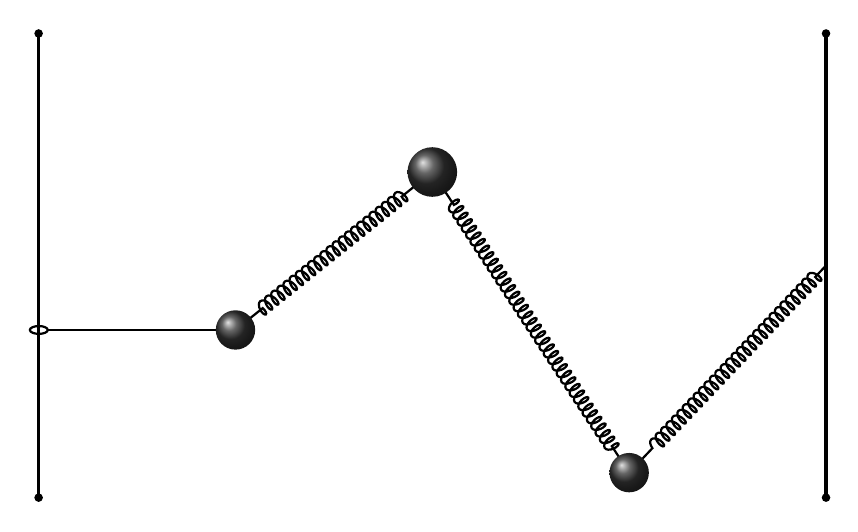
\begin{tikzpicture}
\coordinate (A) at (-2.5,-0.818);
\coordinate (B) at (0,1.188);
\coordinate (C) at (2.5,-2.630);

\draw[very thick,{Circle[length=3pt]}-{Circle[length=3pt]}](-5,-3)--(-5,3);
\draw[very thick,{Circle[length=3pt]}-{Circle[length=3pt]}](5,-3)--(5,3);

\draw[thick,decoration={coil,aspect=-.5,post length=0.35cm,segment length=1mm,pre length=0.5cm},decorate](B)--(A);
\draw[thick,decoration={coil,aspect=-.5,post length=0.35cm,segment length=1mm,pre length=0.5cm},decorate](B)--(C);
\draw[thick,{Ellipse[open]}-](-5.125,0|-A)--(A);
\draw[thick,decoration={coil,aspect=-.5,post length=0.35cm,segment length=1mm,pre length=0.2cm},decorate](5,0)--(C);

\shade[ball color=black!80](A)circle(0.25);
\shade[ball color=black!80](B)circle(0.315);
\shade[ball color=black!80](C)circle(0.25);

\end{tikzpicture}
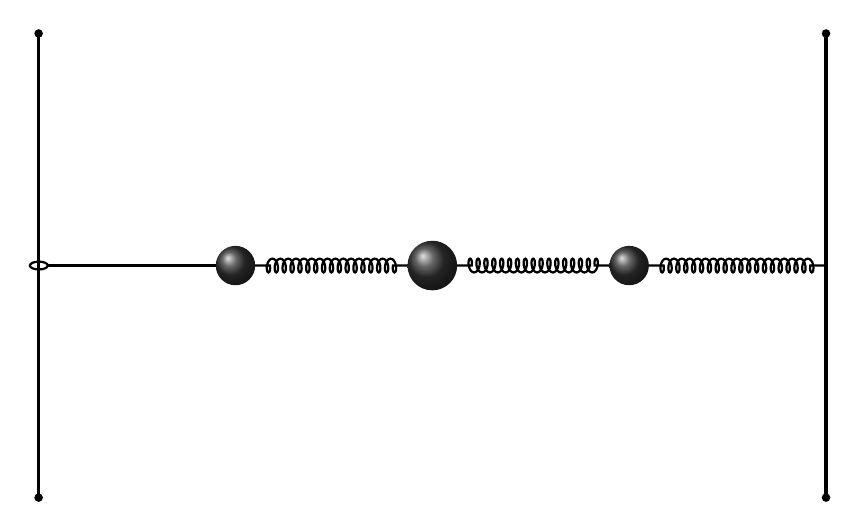
\begin{tikzpicture}
\coordinate (A) at (-2.5,0);
\coordinate (B) at (0,0);
\coordinate (C) at (2.5,0);

\draw[very thick,{Circle[length=3pt]}-{Circle[length=3pt]}](-5,-3)--(-5,3);
\draw[very thick,{Circle[length=3pt]}-{Circle[length=3pt]}](5,-3)--(5,3);

\draw[thick,decoration={coil,aspect=-.5,post length=0.35cm,segment length=1mm,pre length=0.5cm},decorate](B)--(A);
\draw[thick,decoration={coil,aspect=-.5,post length=0.35cm,segment length=1mm,pre length=0.5cm},decorate](B)--(C);
\draw[thick,{Ellipse[open]}-](-5.125,0|-A)--(A);
\draw[thick,decoration={coil,aspect=-.5,post length=0.35cm,segment length=1mm,pre length=0.2cm},decorate](5,0)--(C);

\shade[ball color=black!80](A)circle(0.25);
\shade[ball color=black!80](B)circle(0.315);
\shade[ball color=black!80](C)circle(0.25);

\end{tikzpicture}
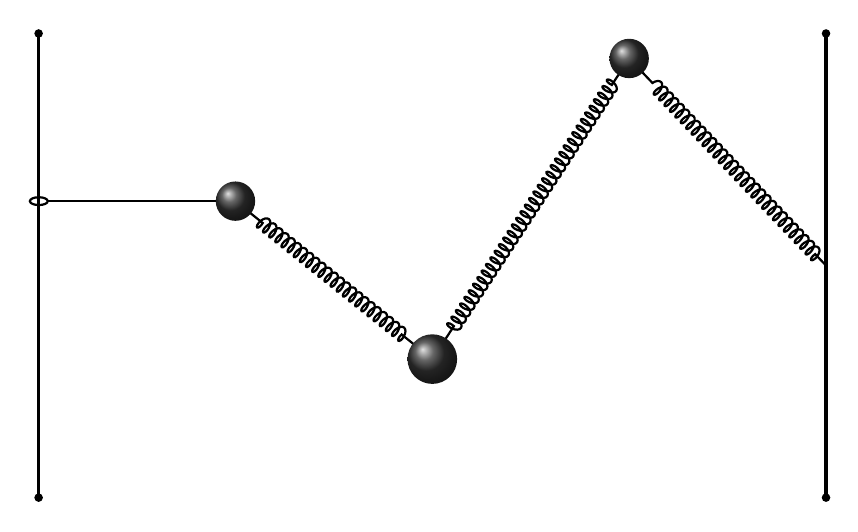
\begin{tikzpicture}
\coordinate (A) at (-2.5,0.818);
\coordinate (B) at (0,-1.188);
\coordinate (C) at (2.5,2.630);

\draw[very thick,{Circle[length=3pt]}-{Circle[length=3pt]}](-5,-3)--(-5,3);
\draw[very thick,{Circle[length=3pt]}-{Circle[length=3pt]}](5,-3)--(5,3);

\draw[thick,decoration={coil,aspect=-.5,post length=0.35cm,segment length=1mm,pre length=0.5cm},decorate](B)--(A);
\draw[thick,decoration={coil,aspect=-.5,post length=0.35cm,segment length=1mm,pre length=0.5cm},decorate](B)--(C);
\draw[thick,{Ellipse[open]}-](-5.125,0|-A)--(A);
\draw[thick,decoration={coil,aspect=-.5,post length=0.35cm,segment length=1mm,pre length=0.2cm},decorate](5,0)--(C);

\shade[ball color=black!80](A)circle(0.25);
\shade[ball color=black!80](B)circle(0.315);
\shade[ball color=black!80](C)circle(0.25);

\end{tikzpicture}
\end{document}